\documentclass[11pt,a4paper]{article}
\usepackage[T1]{fontenc}
\usepackage[utf8]{inputenc}
\usepackage[french]{babel}
\usepackage{booktabs,longtable,array}
\usepackage[a4paper,margin=2.4cm]{geometry}
\usepackage{graphicx}
\usepackage[hidelinks]{hyperref}
\usepackage{microtype}
\setlength{\parindent}{0pt}
\setlength{\parskip}{0.55em}

\title{Résultats négatifs et réfutations partielles du modèle M2}
\author{Réplication computationnelle indépendante}
\date{3 juillet 2026}

\begin{document}
\maketitle

\begin{abstract}
Ce rapport rassemble les échecs qui pourraient être masqués par la présence
visuelle d'une queue droite en échelle log--log. Le corps exponentiel est rejeté,
la Pareto n'est pas distinguée d'une log-normale tronquée, la queue et les classes
dynamiques survivent sans crédit, la population n'est pas robuste aux paramètres
de naissance et aucun signal convaincant de SOC n'est observé. Un artefact
numérique de fractionnement des contrats a également été découvert et corrigé.
Ces résultats n'annulent pas tout intérêt de M2 : ils restreignent son
interprétation à un processus multiplicatif avec absorption et sélection
démographique, dont le réseau de crédit module les niveaux sans être la cause
démontrée de la forme.
\end{abstract}

\section{Objectif et méthode}

L'objectif est de pré-enregistrer les conclusions défavorables avec le même
niveau de visibilité que les résultats positifs. Les preuves proviennent de
trois baselines de 2000 pas, d'une grille de 36 cas à 600 pas, d'ablations courtes
et d'une ablation sans crédit de 2000 pas. Les méthodes statistiques et limites
sont détaillées dans le rapport de validation.

\section{Tableau des verdicts}

\begin{longtable}{p{0.29\textwidth}p{0.18\textwidth}p{0.44\textwidth}}
\toprule
Hypothèse & Verdict & Élément discriminant \\
\midrule
\endhead
Corps exponentiel de NW & Réfutée à l'horizon testé & Fisk gagne les trois seeds ;
$\Delta$AIC exponentielle 61--80 ; zéro victoire sur 36 cas de grille. \\
Température $T=B_0/A_0$ & Non soutenue & Drift moyen des survivants du corps
positif, donc $A_0<0$ avec la convention du rapport. \\
Queue de Pareto stable & Non établie & Seed 2 : $\alpha=2{,}54\to3{,}05$ et
$x_{\min}=324\to857$ ; log-normale tronquée toujours meilleure en vraisemblance. \\
Même queue pour revenu et NW & Réfutée & Exposant revenu 4,20--4,86 contre NW
2,54--3,05. \\
Classes non démographiques & Soutenue & Corrélation âge--log NW 0,064--0,155 ;
mortalité du top 86--91\,\% ; renouvellement presque total. \\
Crédit nécessaire à la queue & Réfutée & Sans crédit à 2000 pas : corps Fisk,
$\alpha=2{,}72/2{,}90/2{,}84$, classes dynamiques. \\
SOC du crédit stabilisant $\alpha$ & Non soutenue & Pas de transition claire en
$k$, tailles de lots similaires, concentration non positivement liée aux morts,
signatures maintenues sans crédit. \\
Population robustement bornée & Non établie & Quasi-plateau baseline mais pentes
positives ; à $\sigma=0{,}15$ certains cas ont 0--5 morts et croissance quasi
linéaire. \\
Absence de réglage fin & Réfutée partiellement & Mortalité et croissance varient
fortement avec $\sigma$ et $\varepsilon_0/w_0$. \\
\bottomrule
\end{longtable}

\section{Le corps exponentiel n'apparaît pas}

Le ratio médiane/moyenne de NW, 0,662--0,676, pourrait suggérer
$\ln2\simeq0{,}693$. Mais un ratio scalaire ne teste pas la forme. Les
vraisemblances tronquées donnent Fisk devant l'exponentielle de 61 à 80 points
d'AIC. Les QQ-plots présentent une courbure. Le résultat se reproduit dans toute
la grille courte : 35 corps Fisk et un log-normal.

\begin{figure}[ht]
\centering
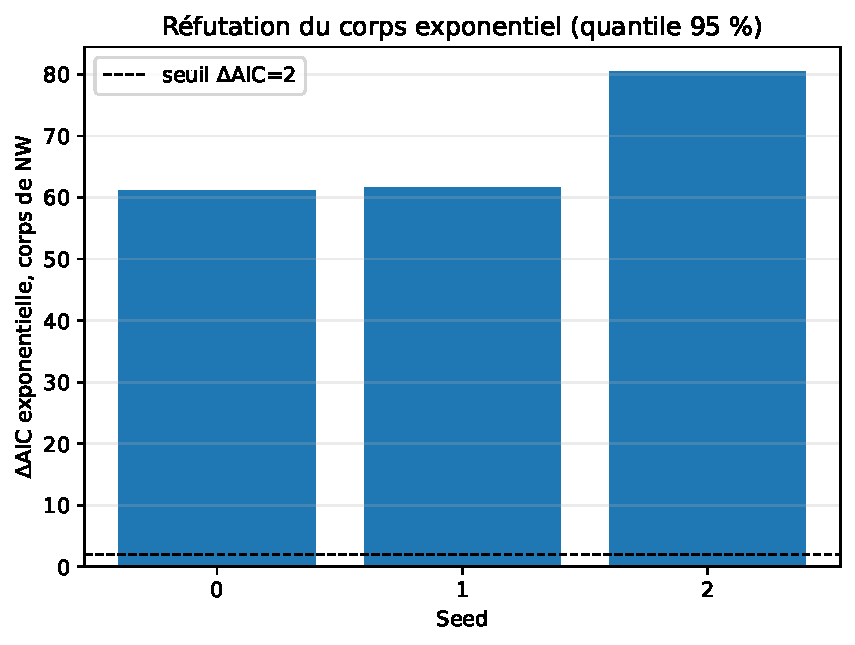
\includegraphics[width=0.67\textwidth]{../04_validation_report/figures/body_exponential_delta_aic.pdf}
\caption{Écart à l'exponentielle pour les trois seeds.}
\end{figure}

Une explication alternative cohérente est le rappel créé par extraction et
dépréciation, combiné à une injection ponctuelle et à un mélange d'états de
bilan. Les transferts de crédit ne réalisent pas un échange additif aléatoire
symétrique de type Boltzmann. Renforcer artificiellement le churn pour améliorer
la forme serait un nouveau paramétrage, pas une validation de M2.

\section{La Pareto est confondue avec une log-normale}

Les exposants proches de 2,8 sont visuellement convaincants. Pourtant, une
log-normale ajustée et normalisée sur le même domaine de queue obtient une
vraisemblance supérieure dans les 27 comparaisons (trois variables, trois seeds,
trois fenêtres). Pour NW, le seed 2 favorise significativement la log-normale en
première fenêtre. Le choix libre de $x_{\min}$ y produit aussi le saut annoncé
comme risque dans le rapport.

Le grand LR favorable à Pareto rapporté par le prototype provenait en partie
d'une comparaison asymétrique : densité Pareto conditionnée à $x_{\min}$ contre
densité log-normale non renormalisée après sélection de la queue. La correction
ne prouve pas que la loi est log-normale ; elle supprime la preuve alléguée en
faveur de Pareto.

\section{L'explication SOC ne résiste pas aux ablations}

\begin{figure}[ht]
\centering
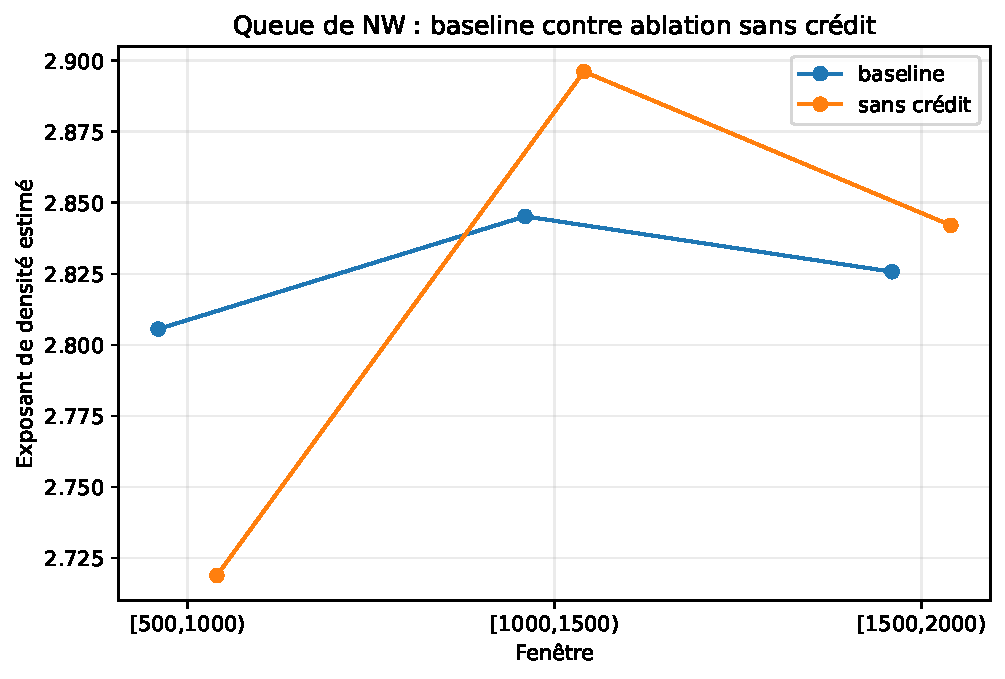
\includegraphics[width=0.72\textwidth]{../04_validation_report/figures/baseline_vs_no_credit_tail.pdf}
\caption{Exposants de NW avec et sans réseau de crédit.}
\end{figure}

Supprimer tout crédit laisse le choc multiplicatif sur $w$, l'extraction, la
dépréciation, $d_0$, l'absorption et la réinjection. Cette ablation conserve la
queue apparente, le corps Fisk et le renouvellement social. Elle isole un
processus proche de Kesten avec seuil de mort ; c'est une explication plus simple
que la stabilisation par cascades de crédit.

Les lots de faillites ont une moyenne 7,7--8,0 et un maximum 18--22 pour
$k=2,3,4,6$. Leur plage est trop courte pour soutenir une loi d'échelle et aucune
bifurcation $k\geq3$ n'est visible. La corrélation de rang entre concentration du
crédit au pas précédent et faillites vaut de $-0{,}23$ à 0. Ce diagnostic ne
permet pas une revendication SOC.

\section{Le bornage dépend fortement de la fenêtre de naissance}

\begin{figure}[ht]
\centering
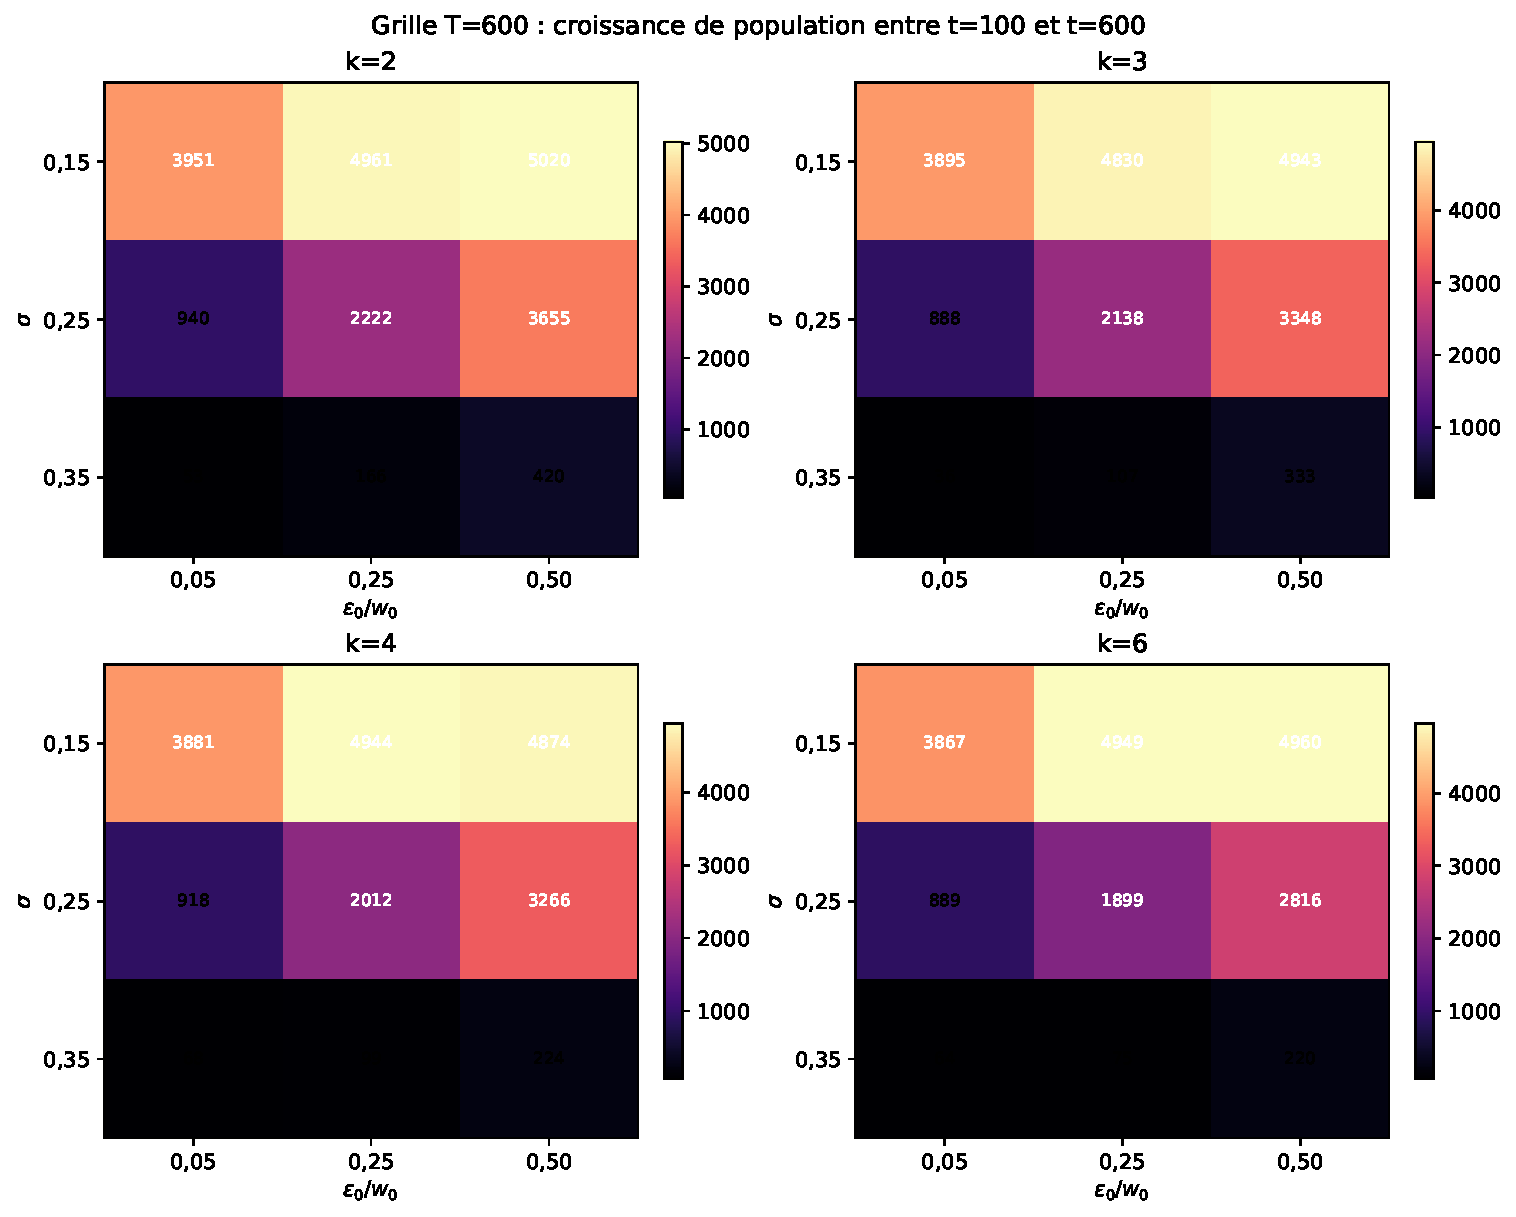
\includegraphics[width=0.9\textwidth]{../04_validation_report/figures/grid_population_growth.pdf}
\caption{Croissance sur 500 pas pour les 36 cas de la grille.}
\end{figure}

Le régime baseline ralentit vers $N\simeq1670$, mais conserve une pente positive
sur $[1000,2000]$. Dans la grille, diminuer $\sigma$ ou augmenter la marge de
naissance supprime presque la mortalité et restaure $N(t)\simeq\lambda t$. La
condition de fenêtre n'est donc pas une simple cohérence dimensionnelle : c'est
un réglage de l'existence du régime. Une robustesse sans réglage fin n'est pas
observée.

\section{Artefact numérique découvert}

Le transfert récursif au prorata a fait croître le nombre de fragments de 3482 à
142766 entre $t=1200$ et $t=1414$, avec 588 Mo de mémoire avant interruption.
Une simulation naïve aurait pu s'arrêter ou devenir dépendante d'un epsilon de
suppression des petits contrats. La fusion exacte par paire évite cet artefact
sans seuil et conserve les flux. Ce résultat montre que la règle prorata possède
une complexité cachée absente du prototype, lequel annulait simplement les
créances de la faillie.

\section{Résultats positifs qui subsistent}

Le résultat anti-cohorte est solide : aucune cohorte fondatrice immortelle, top
fortement renouvelé et faibles corrélations d'âge. Le modèle produit aussi une
mortalité endogène et un régime démographique de taille finie sur la baseline,
sans capacité de charge. Enfin, les exposants au seuil commun sont moins
instables que les estimations libres. Ces points sont des propriétés numériques
reproductibles, mais ils ne suffisent ni à une loi Boltzmann--Pareto ni à une SOC.

\section{Limites et prochaines expériences}

Le verdict reste conditionnel à trois seeds et 2000 pas. Les lots de faillites ne
sont pas des avalanches causales. Les estimations d'incréments omettent les morts
entre snapshots. La grille est courte et mono-seed. Les prochaines expériences
doivent donc prolonger baseline et sans crédit, répéter les frontières de grille,
construire un protocole d'avalanches séparant forçage et relaxation, et comparer
les lois en prédiction hors échantillon.

Une variante ne doit être introduite que pour tester une cause précise. Changer
la moyenne des taux, augmenter les rounds ou modifier la liquidation après
inspection du corps constituerait une nouvelle version M3 ; cela ne doit pas être
présenté comme succès de M2.

\section{Conclusion}

Le résultat le plus vrai et utile est négatif : M2 n'a pas produit la
distribution Boltzmann--Pareto revendiquée selon les critères stricts du rapport,
et le mécanisme SOC n'est pas nécessaire aux signatures observées. Le modèle
réussit le garde-fou démographique et reste une plateforme testable pour étudier
absorption, renouvellement et crédit. Toute suite doit partir de ce verdict, non
du seul aspect rectiligne des queues.

\end{document}
